% !TEX root = ../Masterarbeit.tex
\chapter{Grundlagen \& Begriffsbestimmung}
In diesem Kaptiel werden die Grundlagen geschaffen, auf die der Hauptteil aufbaut. Zudem behandelt das Kapitel die Begriffsbestimmung und die genauen Eigenschaften reaktiver Systeme.\\
Da die Umsetzung reaktiver Systeme gewisse Programmierparadigmen vorausgesetzt, werden diese nach den reaktiven Merkmalen erklärt.

\section{Eigenschaften reaktiver Systeme}
Reaktive Anwendungen haben die Eigenschaften folgendes zu leisten bzw. foldenge Punkte zu erfüllen~\cite[S.~19ff]{kuhn_reactive_2015}~\cite[S.~6]{vernon_reactive_2016}.\\

\textbf{Eine reaktive Anwendung muss\ldots}
\begin{enumerate}
\item \ldots \textbf{auf variable Belastung reagieren (siehe~\ref{subsec:elastic}.).} Das System ist automatisch in der Lage dynamische Skalierung durchzuführen und nicht benötigte Ressourcen wieder freizugeben.
\item \ldots \textbf{auf Fehler reagieren (siehe~\ref{subsec:resilient}).} Die Software ist von Grund auf widerständsfähig gegenüber Fehlerzuständen. Die Wiederherstellung des Normalzustand erfolgt automatisch.
\item \ldots \textbf{auf Nutzer oder Komponenten reagieren (siehe~\ref{subsec:responsive}).} Jede Anfrage wird in der geforderte Antwortzeit bearbeitet und übertrifft diese eventuell sogar.
\item \ldots \textbf{auf Nachrichten reagieren (siehe~\ref{subsec:messagedriven}).} Das System verwendet asynchrone Nachrichtenübermittlung zwischen den Komponenten und ist somit \textit{message-driven}.
\end{enumerate}

Die nachfolgenden Abschnitte erklären die Merkmale im Detail und zeigen den Zusammenhang zwischen ihnen.

\subsection{Elastic}\label{subsec:elastic}
Eine reaktive Anwendung muss auf variable Belastung ebenso variable bzw. dynamisch reagieren können. Wird Beispielsweise ein Online Shop in einer Fernsehwerbung oder von einem bekannten Blog erwährt, müssen kurzfristig sehr viele Anfragen angemessen und zufriedenstellend verarbeitet werden~\cite[S.~39]{kuhn_reactive_2015}.\\
Um die gewünschten und geforderten Antwortzeiten einzuhalten, muss das System skalieren. Traditionellerweise ist hiermit \textit{scaling up} gemeint. Aufgrund der heutigen Anforderungen stößt man schnell an die Grenzen eines einzelnen Hosts. Dementsprechend muss das System nicht nur vertikal sondern auch horizontal skalieren. Dazu muss das System auf mehrere Nodes verteilt werden~\cite[S.~7]{vernon_reactive_2016}. Es ist deshalb wichtig, die Teilaufgaben eines Systems zu identifizieren und auf einzelne Komponenten aufzuteilen, die dann wie bereits erwähnt auf einzelne Nodes verteilt werden können~\cite[S.~40]{kuhn_reactive_2015}.\\
Das Reactive Manifesto fordert zudem auch, das System so zu gestalten, dass es \textit{scaling down} fähig ist. Das bedeutet ungenutze und nicht benötigte Ressourcen müssen wieder freigegeben werden. Dadurch kann man ein hochskalierbares reaktives System kosteneffizient betreiben. Im Reactive Manifesto hat man sich auf den Begriff \textit{elastic} geeinigt, um deutlich zu machen, dass man in beide Richtungen skalieren kann. Bei reaktiven Applikationen spricht man deshalb von elastischer bzw. dymanischer Skalierung~\cite[S.~8]{vernon_reactive_2016}. Für die Software bedeutet dies, dass einzelne Nodes jederzeit hinzugefügt und entfernt werden können. Als Folge dessen muss das System \textit{location transparent} sein. Insofern dürfen dessen Komponenten und Funktionen nicht abhängig von einem Host sein~\cite[S.~8]{vernon_reactive_2016}. 

% TODO Little's Law
% TODO Infrastructure as a Service oder Cloud Computing; Enterprise IT OpenStack

\pagebreak

\subsection{Resilient}\label{subsec:resilient}
Eine Software \textit{resilient} (dt. widerstandsfähig) zu entwickeln bedeutet nicht, dass die Software fehlerfrei ist. Es bedeutet, dass die Software sich von einem Fehlerzustand erholen kann~\cite[S.~6]{vernon_reactive_2016}.\\
Man versucht bei dem Entwurf der Software Fehler von vornherein zu bedenken und mit ihnen sinnvoll umzugehen. Folgendes Zitat von Jonas Bonér macht deutlich, wie wichtig die Widerstandsfähigkeit einer Software ist.

\begin{quotation}
Without resilience, nothing else matters. If your beautiful, production-grade, elastic, scalable, highly concurrent, non-blocking, asynchronous, highly responsive and performant application isn't running, then you're back to square one. It starts and ends with resilience.~\citetext{Bonér, Jonas; 2015}
\end{quotation}

Im Grunde ist diese Aussage trivial. Eine Software die nicht läuft, ist unbrauchbar --- egal wie komplex und durchdacht die Architektur auch sein mag.\\
Es ist aber nicht nur die eigene Software, die betroffen sein kann. Andere externe Softwarekomponenten von denen man abhängt oder auch die Hardware kann im laufenden Betrieb Probleme bereiten~\cite[S.~33]{kuhn_reactive_2015}.\\
Der Schluss, den man daraus ziehen sollte, lautet deshalb nicht, ob ein Fehler auftritt sondern viel mehr wann und wie häufig das passiert. Für den Benutzer ist es nebensächlich warum ein interner Fehler aufgetreten ist. Die Anwendung wird in diesem Moment nicht das tun, was der Benutzer von ihr erwartet~\cite[S.~33]{kuhn_reactive_2015}.\\

Im Reactive Manifesto hat man für dieses Problem bzw. die Eigenschaft ganz bewusst den Begriff \textit{resilience} und nicht \textit{reliability} (dt. Ausfallsicherheit) gewählt. Man möchte deutlich machen, dass es nahezu unmöglich ist, ein ausfallsicheres System zu schaffen. Deshalb setzt man auf widerstandsfähige Systeme, welche mit Fehlerzuständen sinnvoll umgehen und vorallem sich von dieses wieder erholen. Folglich ist ein reaktives System nicht nur \textit{fault tolerant} (dt. Fehler tolerant) sondern geht noch einen Schritt weiter~\cite[S.~34]{kuhn_reactive_2015}.\\

Um die Eigenschaft \textit{resilience} zu erfüllen, muss das System in Komponenten aufgeteilt und anschließend verteilen (engl.~\textit{distribute}) werden. Zusätzlich ist es notwendig die verteilen Komponenten von einander abzuschotten (engl.~\textit{compartmentalize})~\cite[S.~34]{kuhn_reactive_2015}~\cite[S.~7]{vernon_reactive_2016}.\\
Aufgrund der verteilten und abgeschottenten Komponenten können Fehler isoliert werden. Hierfür führt man das Prinzip der \textit{supervision} ein. Nach- bzw. untergeordnete Komponenten informieren ihren \textit{supervisor} im Falle eines Fehlers. Dieser hat nun die Möglichkeit die Subkomponente z.B. neuzustarten oder eine erneute Anfrage zustellen. 

\subsection{Responsive}\label{subsec:responsive}
Eine reaktive Anwendung muss zu jederzeit auf jede Anfragen reagieren. Das heißt die Anwendung ist jederzeit \textit{responsive} (dt. antwortbereit). Anfragen können nicht nur durch einen Benutzer ausgelöst werden, sondern können auch von anderen Diensten oder Komponenten initiert werden. Als Client einer reaktiven Anwendung muss man sich drauf verlassen können, dass eine Antwort in einem festgelegten Zeitraum eintrifft. Das bedeutet es müssen \textit{timeouts} festgelegt werden, nachdem eine Anfrage für fehlerhaft erklärt wird.\\
Ist eine Anwendung nicht \textit{elastic} (siehe~\ref{subsec:elastic}) und/oder nicht \textit{resilient} (siehe~\ref{subsec:resilient}) kann sie auch nicht \textit{responsive} sein. Eine reaktive Anwendung muss unter Last skalieren, um die geforderte maximale Antwortzeit einzuhalten oder zu vermeiden, dass das System ganz ausfällt. Gleichzeitig eingehende Anfragen müssen parallel verarbeitet werden können und dürfen nicht von langsamen Anfragen blockiert werden.Fallen Komponenten aus, z.B. durch einen unvorhergesehenen Hardwarefehler, könnten diese aufgrund der \textit{location transparency} auf einem anderen Node neu gestartet werden, um die \textit{responsivenes} aufrechtzuerhalten.

\pagebreak

\subsection{Message-driven}\label{subsec:messagedriven}
Um die bereits erwähnten Eigenschaften \textit{elasticity} (\ref{subsec:elastic}), \textit{resilience} (\ref{subsec:resilient}), sowie die daraus folgende \textit{responsiveness} (\ref{subsec:responsive}) zu erfüllen, müssen reaktive Anwendungen \textit{message-driven} sein~\cite{webber_what_2014}~\cite[S.~43]{kuhn_reactive_2015}. Somit ist die Basis einer reaktiven Anwendung die vierte Eigenschaft aus dem Reactive Manifesto~\cite{boner_reactive_2014}.\\
Ist ein System \textit{message-driven} erfolgt die Kommunikation ausschließlich über asynchronen Nachrichtenaustausch zwischen den Komponenten, wodurch eine strikte Abgrenzung der Komponenten erfolgt. Durch die Abstraktion der Kommunikation wird eine lose Kopplung zwischen den Komponenten sichergestellt. Darüber hinaus sind die Komponenten voneinander isoliert, wodurch es möglich ist, Fehler als Nachrichten zu delegieren (siehe~\ref{subsec:resilient}).\\
Durch den expliziten Nachrichtenaustausch kann über \textit{message queues} und \textit{flow control} die Last verteilt und kontrolliert werden. Ebenso wird die gewünschte \textit{location transparency} durch die Entkopplung über den asynchronen Nachrichtenaustausch ermöglicht~\cite{boner_reactive_2015}~\cite[S.~43]{kuhn_reactive_2015}.\\
Die folgende Abbildung (Abb. \ref{fig:four-traits}) soll den Zusammenhang der vier Merkmale nochmals verdeutlichen. Neben dem wohl wichtigsten Ziel der \textit{responsiveness} hat die reaktive Architektur den Vorteil wartbare und auch erweiterbare Anwendungen zu schaffen. Jedoch werde die weiteren Ziele nur in der Einleitung des Reactive Manifestos und nicht als Kerneigenschaft formuliert~\cite{boner_reactive_2014}. Die Ziele erreicht man durch die Eigenschaften \textit{elasticity} und \textit{resilience}. Die Grundvoraussetzung ist im wesentlichen die asynchrone, nicht-blockierende und nachrichtengetriebene Kommunikation (\textit{message-driven}).

\begin{figure}[H]
 \centering
 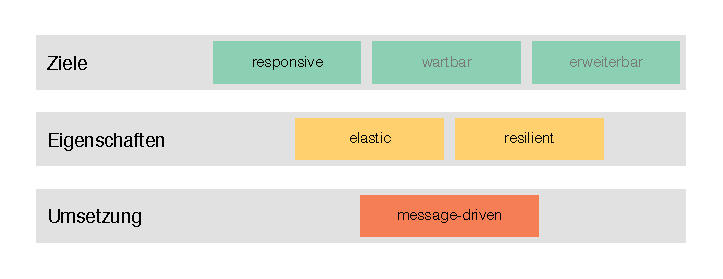
\includegraphics[width=1.0\textwidth]{3-Grundlagen/four-traits/four-traits.eps}
 \caption{Die vier Merkmale einer reaktiven Anwendung \cite{kuhn_code_2015}}
 \label{fig:four-traits}
\end{figure}

\pagebreak

\section{Parallelität und Nebenläufigkeit}
Die Prozessorhersteller sind in den letzten Jahren an gewisse Grenzen bei der Entwicklung von CPUs gestoßen. Seit 2003 stagniert die Entwicklung hinsichtlich der Taktraten von Prozessoren. Obwohl die Beobachtung von Gordon Moore (\enquote{Moore's Law}) nach wie vor seine Gültigkeit zu haben scheint und sich die Zahl der Transistoren alle zwei Jahre verdoppelt, werde diese nicht genutzt, um eine einzelne CPU schneller zu machen. Hersteller setzen stattdessen seit einigen Jahren auf Multicore-Architekturen~\cite[S.~1]{butcher_seven_2014}~\cite[S.~108]{vernon_reactive_2016}~\cite{sutter_free_2004}.\\
Herb Sutter veröffentlichte diesbezüglich 2004 einen Artikel mit dem Titel \enquote{The free lunch is over}. Mit \enquote{free lunch} bezog er sich auf die Tatsache, dass sequenzielle Anwendungen ohne das Zutun von Entwicklern aufgrund der damals noch steigenden Taktraten schneller wurden --- vielmehr schneller ausgeführt wurden.\\
Im Hinblick auf die Multicore-Prozessoren und der mehr oder weniger stagnierenden Taktraten müssen Anwendungen ihre Aufgaben und Teilaufgaben nebenläufig und parallel ausführen, um die heutigen und zukünftigen Prozessoren optimal auszulasten~\cite{sutter_free_2004}~\cite[S.~1]{butcher_seven_2014}.\\
Sequenzielle Programme werden Schritt für Schritt ausgeführt. Genauer gesagt, erfolgt die Ausführung der einzelnen Befehle nach einer vorgegebenen Reihenfolge. Folglich profitiert ein sequenzielles Programm nicht von modernen Multicore-Prozessoren. Hier kommen nun Nebenläufigkeit (engl. concurrency) und Parallelität (engl. parallelism) ins Spiel~\cite[S.~3]{butcher_seven_2014}.\\

Die Welt in der wir leben ist hochgradig parallel. Während man Auto fährt, nimmt man, wenn auch  meist unterbewusst, viele unterschiedliche Dinge gleichzeitig wahr. Während man sich sportlich betätigt, hört man gleichzeitig zum Laufen noch Musik, um sich anzuspornen. Während man seinem Smartphone mit dem Finger sagt was es tun soll, kann man trotzdem derweil Emails empfangen.\\
In Hinblick auf Prozessoren und Software muss man zwischen mehreren Ebenen von Parallelität unterscheiden. Zum Beispiel kann ein Singlecore-Prozessor aufgrund von Technologien wie Pipelining mehrere Schritte parallelisieren. Ebenso sind Multitasking Betriebssysteme in der Lage auf einem Singlecore-Prozessor mehrere Prozesse nebenläufig bzw. quasi-parallel auszuführen~\cite[S.~3~\&~S.~4]{butcher_seven_2014}. Der folgende Abschnitt bezieht sich auf Parallelität im Bezug auf Multicore-Prozessoren und wie diese erreicht werden kann.\\
Nebenläufigkeit und Parallelität werden fälschlicherweise oft als Synonyme verwendet. Die beiden Begriffe sind verwandt, beschreiben jedoch verschiedene Sachverhalte. Eine nebenläufige Applikation besitzt mehrere logische Threads (\textit{threads of control}). Diese können aber müssen nicht parallel ausgeführt werden. Eine parallele Anwendung berechnet Ergebnisse eventuell schneller als eine sequenzielle Anwendung durch die gleichzeitige Ausführung von Teilproblemen. Meist gibt es dann jedoch nur einen logischen Thread~\cite[S.~1]{butcher_seven_2014}.\\
Betrachtet man Nebenläufigkeit und Parallelität aus der Sicht eines Problems (Problemdomäne), bedeutet Nebenläufigkeit das Bearbeiten gleichzeitig oder annähernd gleichzeitig eintreffender Ereignisse. Im Gegensatz dazu bezieht sich Parallelität auf die beschleunigte Lösung eines Problems durch Fragmentierung und der simultanen Bearbeitung der Teilprobleme~\cite[S.~2]{butcher_seven_2014}~\cite[S.~15]{vernon_reactive_2016}.\\
Rob Pike formulierte den Unterschied zwischen Nebenläufigkeit und Parallelität wie folgt:

\begin{quotation}
  Concurrency is about dealing with lots of things at once. Parallelism is about doing lots of things at once. [...] Concurrency provides a way to structure a solution to solve a problem that may (but not necessarily) be parallelizable~.
\cite[S.~10]{pike_concurrency_2012}
\end{quotation}

Nebenläufigkeit beschreibt die Koordination mehrerer unabhängiger Abläufe. Parallelität hingegen die simultane bzw. gleichzeitige Ausführung von Berechnungen, die nicht zwingendermaßen zusammenhängen~\cite[S.~8-9]{pike_concurrency_2012}~\cite[S.~3]{butcher_seven_2014}.\\
Kann ein Problem bzw. eine Anwendung nebenläufig beschrieben bzw. entworfen werden, ist es möglich, die Anwendung parallel und entsprechend schneller auszuführen~\cite[S.~19~\&~S.~30]{pike_concurrency_2012}. Gene Amdahl stelle hierfür bereits 1967 ein Modell auf (\enquote{Amdahl's Law}). Das Modell beschreibt den Grad der Beschleunigung einer Anwendungen durch dessen parallele Anteile. So kann eine Anwendung, die nur zu 90~\% parallelisiert ist, maximal um den Faktor 10 schneller ausgeführt werden~\cite{amdahl_validity_1967}.\\

Die Art und Weise, wie wir heute mit der digitalen Welt interagieren, ist nebenläufig und parallel. Demnach müssen Anwendungen ebenso nebenläufig sein, um den Anforderungen zu entsprechen~\cite[S.~5]{butcher_seven_2014}~\cite[S.~3]{armstrong_programming_2013}.\\
Ein nebenläufiges Design erlaubt es einer Anwendung \textit{responsive}, fehlertolerant und effizient zu sein~\cite[S.~4~\&~S.~6]{butcher_seven_2014}~\cite[S.~6]{armstrong_programming_2013}.\\
Nur eine Anwendung, die nebenläufig mehrere Ereignisse verarbeiten kann, ist in der Lage \textit{responsive} zu sein. Beispielsweise kann ein Browser mehrere Webseiten gleichzeitig (nebenläufig) laden und der Benutzer hat die Möglichkeit währenddessen eine weitere Seite zu öffnen, ohne auf die Beendigung der anderen Ladevorgänge warten zu müssen. Verteilt man eine Anwendung auf mehrere Nodes, muss diese implizit nebenläufig sein --- oder anders ausgedrückt, nebenläufiges Design erlaubt das Verteilen auf mehreren Nodes. Die Möglichkeit eine Anwendung zu verteilen und somit redundant zu betreiben, ist Basis für \textit{resilience} und \textit{elasticity}~\cite[S.~6]{butcher_seven_2014}~\cite[S.~6~\&~S.~7]{armstrong_programming_2013}.\\

Zusammenfassend kann man diesem Abschnitt entnehmen, dass reaktive Anwendungen per Definition nebenläufig entworfen und umgesetzt werden müssen, um die Eigenschaften des Reactive Manifestos erfüllen zu können.

\pagebreak

\subsection{Responsivness in synchronen Anwendungen}
Die einfachste Kommunikation zwischen zwei Komponenten ist die synchrone Kommunikation. Komponente \textit{a} ruft eine Funktion \textit{f} der Komponente \textit{b} auf. Die Berechnung erfolgt synchron und deshalb wartet Komponente \textit{a} auf das Ergebnis und kann dann erst die weiteren Schritte sequenziell abarbeiten. Die weiteren Schritte müssen jedoch nicht bedingt von dem Ergebnis der Funktion \textit{f} abhängig sein. Sollte bei dem Funktionsaufruf ein Fehler auftreten, werden die nachfolgenden Befehle nicht ausgeführt. Jedoch ist Komponente \textit{b} von diesem Fehler betroffen, solange die beiden Komponenten im gleichen Thread ausgeführt werden. Komponente \textit{a} und \textit{b} sind stark voneinander abhängig~\cite[S.~22]{kuhn_reactive_2015}.\\
Sobald die Komponenten \textit{a} und \textit{b} verteilt werden, löst sich die Kopplung. Dies kann durch Ausführung in jeweils eigenen Threads geschehen oder durch die Verteilung auf mehrere Nodes und die Kommunikation über das Netzwerk.\\

%TODO Waldo et al \enquote{A Note on Distributed Computing}\\
%TODO Deutsch et al \enquote{Fallacies of Distributed Computing}

\subsection{Asynchronous \& Non-Blocking IO}
Ein wichtiger Schritt zu einer reaktiven Anwendung impliziert verteilte und isolierte Komponenten. Es ist nicht zwingend erforderlich, dass die Komponenten auf verschiedenen Hosts laufen und dennoch ist dies aufgrund der \textit{location transparency} möglich. Selbst auf einem Node mit lokaler Kommunikation hat man Latenzen. In traditionellen Applikationen wartet eine Komponente auf die Antwort einer angefragten Komponente. Man spricht hier von synchroner und blockierender (eng. \textit{blocking}) Kommunikation. Das System muss warten und Ressourcen (z.B. CPU) werden nicht optimal genutzt. Darunter leidet dann die \textit{responsiveness}.

%(Beispiel typischer Applicationcontainer mit 20 Threads)

\subsection{Share nothing}
Da einzelne Komponenten voneinander isoliert sein müssen, dürfen sie auch keinen \textit{state} bzw. keine Informationen teilen. Die Komponenten haben somit keinen \textit{shared memory}. Ein reaktives System fordert die Komponenten dazu auf, zu kommunizieren, um Informationen auszutauschen. In einem \textit{message driven} System werden Nachrichten verschickt, um Komponenten über z.B. eine Zustandsänderung zu informieren.\\
Durch diese klare Entkopplung erhält man ebenso klare Grenzen zwischen den Komponenten. Dies führt zu Kapselung von Fehlern, Implementierungsdetails und Verantwortlichkeiten.

% TODO solution for this: reactive manifesto & actor model

\pagebreak

\section{Functional programming}
In traditioneller sequentieller Programmierung nutzt man so genannten \textit{mutable state}. Also ein Zustand bzw. eine Variable, die jederzeit verändert werden kann. Da reaktive Anwendungen nebenläufig ausgeführt werden, muss der Zugriff auf \textit{mutable state} synchronisiert werden. Es entstehen ähnliche Probleme wie bei synchroner Kommunikation, teile der Anwendungen müssen warten und somit werden Systemressourcen blockiert.\\
Ist eine Variable \textit{immutable} bedeutet das, sie ist nach dem initialen Setzen eines Wertes nicht mehr veränderbar. Der gleichzeitige Zugriff auf einen \textit{shared immutable state} muss somit nicht mehr synchronisiert werden, da die Variable nur einmal beschrieben werden kann.

% Non-determinism caused by concurrent threads accessing shared mutable state. To get determinism, avoid mutable state. To avoid mutable state it means to program functially.

\section{Reactive programming}
Reaktive Programmierung ist in der Entwicklung von Benutzeroberflächen üblich und verbreitet. Als Entwickler einer GUI stetig auf eingehende Events reagieren (z.B. Cursorbewegung, Tastendruck). Während der Verarbeitung dieser soll die Benutzeroberfläche nicht blockieren und Eingaben dadurch verhindern. Eine Benutzeroberfläche muss responsive sein, um dem Benutzer keinen Ärger zu bereiten.\\

%TODO Nachrichtenstorm\\
%TODO Events: facts about things that have happend

\subsection{Reactive extensions \& Oberservable}
%TODO Rx are libraries for asynchronous and therefore reactive programming.\\
%TODO Evolution: imperative -> functional -> reactive
